\section{Ejemplos}\label{sec:ejemplos}

\begin{frame}
\frametitle{Ejemplos}
Mostrar algunos ejemplos básicos, para que la gente tenga una idea del código que produce distintas cosas, uso de paquetes.

\

Indicar dónde se puede obtener más información sobre cómo escribir cosas con \LaTeX, \href{https://ctan.org/}{CTAN},  documentación de \href{https://www.overleaf.com/learn}{Overleaf}, \href{https://tex.stackexchange.com/}{\TeX{} Stack Exchange}, \href{https://www.latex-project.org/help/documentation/}{The \LaTeX{}   Project}
    
\end{frame}

\begin{frame}[fragile]
\frametitle{Ejemplos}
\framesubtitle{Hola mundo!}

Como es habitual con muchos lenguajes, veamos cómo hacer nuestro "Hola mundo!":

\begin{multicols}{2}
\begin{lstlisting}[title={hola\_mundo.tex}]
\documentclass{article}

\begin{document}

Hola mundo!

\end{document}
\end{lstlisting}

\begin{figure}
hola\_mundo.pdf

\includegraphics[width=0.35\textwidth]{../images/ejemplo_hola_mundo.png}
\end{figure}

\end{multicols}

\end{frame}


\begin{frame}[fragile]
\frametitle{Ejemplos}
\framesubtitle{Armando un TP}

¿Qué podríamos querer hacer?

\begin{lstlisting}[title={segundoTP.tex}]
\documentclass{article}
\title{Tremendo TP}
\author{Nuestro grupo}
\date{23:55 (nos sobraron 5)}

\begin{document}
\maketitle

En este trabajo práctico nos proponemos resolver ...

\end{document}
\end{lstlisting}

\end{frame}

\begin{frame}
\frametitle{Ejemplos}
\framesubtitle{Armando un TP}

\begin{figure}
segundoTP.pdf
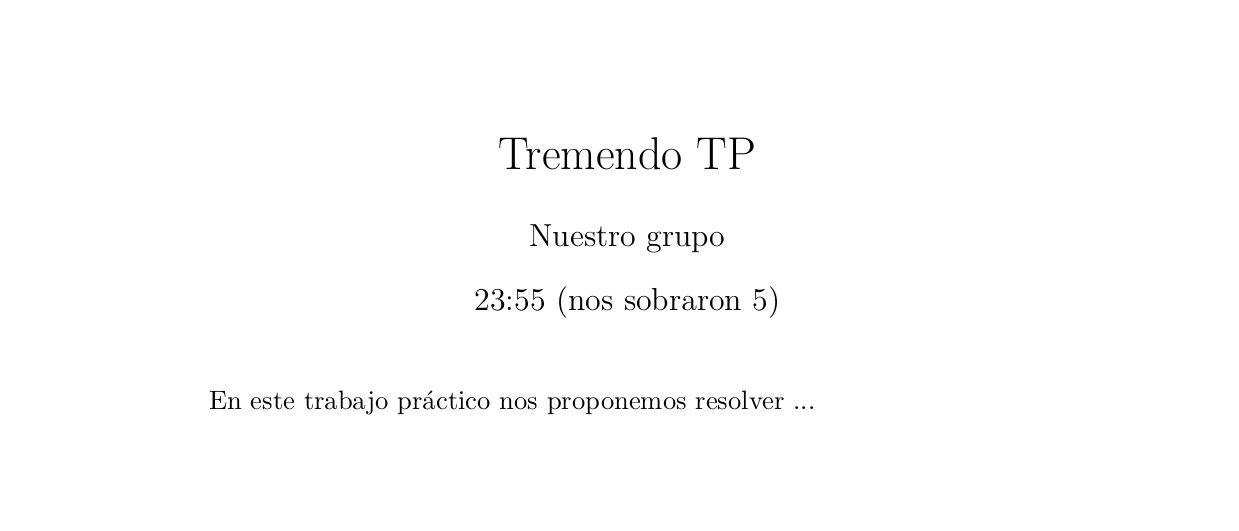
\includegraphics[width=0.9\textwidth]{../images/ejemplo_tp_1.png}
\end{figure}

A su vez, se puede incluir un subtítulo, omitir algunos de los campos, o también usar funciones como \texttt{\textbackslash today} para que la fecha se actualice automáticamente con cada compilación.

\end{frame}

\begin{frame}[containsverbatim]
\frametitle{Ejemplos}
\framesubtitle{Presentaciones}

¿Y si queremos armar slides para una presentación?

\begin{lstlisting}
\documentclass{beamer}
\begin{document}

\begin{frame}[containsverbatim]
\frametitle{Ejemplos}
\framesubtitle{Presentaciones}

¿Y si queremos armar slides para una presentación?

...

\end{frame}

\end{document}
\end{lstlisting}

\end{frame}

\begin{frame}
\frametitle{Ejemplos}
\framesubtitle{Paquetes}

En muchas ocasiones, vamos a querer funcionalidades, entornos, estilos, fuentes, etc. que para utilizarse requieren que usemos el \textbf{paquete} adecuado para ello.

\

Por ejemplo, nos gustaría poder incluir hypervínculos en nuestro documento, de forma que en el contenido del mismo utilice enlaces para acceder a otros documentos o sitios web.
\end{frame}

\begin{frame}
\frametitle{Ejemplos}
\framesubtitle{Paquetes}

Por defecto, tenemos la posibilidad de indicar que algo es una URL. 

Por ejemplo:

\

\begin{center}
\textit{(...)} para más información, consultar la web del departamento de compuntación \url{https://www.dc.uba.ar}.
\end{center}

\pause

Mientras que utilizando el paquete \href{https://ctan.org/pkg/hyperref}{hyperref} podemos escribir lo siguiente


\begin{center}
\textit{(...)} para más información, consultar la web del \href{https://www.dc.uba.ar}{departamento de computación}.
\end{center}

Lo cual resulta más prolijo para enlazar URLs, secciones de un informe, referencias, etc.

\end{frame}
